\begin{figure}
  \centering
  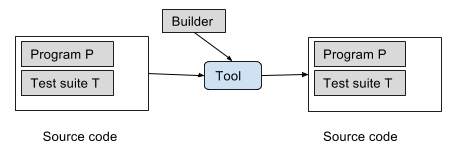
\includegraphics[width=1.0 \columnwidth]{basic_tool_architecture.png}
  \caption{Overview of the tool}
  \captionsetup{justification=centering}
  \label{fig:fig1}
\end{figure}



The basic architecture of the tool from a user's perspective is shown in figure ~\ref{fig:fig1}. For Java-JUnit combo, user just needs to provide the source code that consists of program and labeled tests for java projects.The only extra information needed is build command - ant,gradle or maven command for modern day java projects. No separate mechanism is needed to feed DD with pass-fail result by setting up a tester, running it and collecting the results. 

Figure ~\ref{fig:figDetailedToolArch} describes the detailed architecture of the tool. Components in oval gray are input/output, original program P, Test suite T, and builder constitute input and Program P$'$ is output. Components in white rectangle constitute part of the tool. Architecture follows standard HDD/DD procedure of reduction while taking into account the changes proposed in intuitive modification subsection. Program is passed to AST Parser \cite{javaparser}, we used JavaPaser for this. We implemented our own HDD to reflect changes mentioned in intuitive modification subsection. Similarly, we have our own implementation of DD for the reasons mentioned in intuitive modification subsection. Apart from implementation/algorithmic changes that we proposed, the major architectural change consists of how test results are being fed to dd. Tools like picireny and chipperJ require some sort of test script and pre-processing for developers, while testing is built in as part of our tool. 			

\begin{figure*}
  \centering
  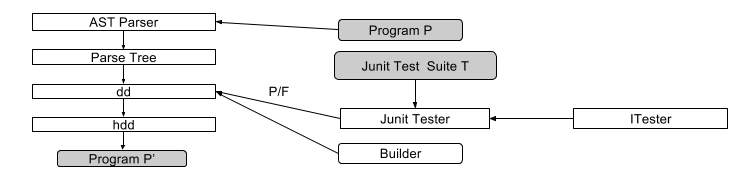
\includegraphics[width=1.8 \columnwidth]{detailed_tool_architecture.png}
  \caption{Architecture of the tool}
  \captionsetup{justification=centering}
  \label{fig:figDetailedToolArch}
\end{figure*}